%{\bf BME154L - Spring 2012 - Exam \#2 Solutions}\hfill Name (Net ID):\underline{\hspace*{3.0in}}



\section*{Optional Problem: Filter Design [2 points]}
\begin{center}
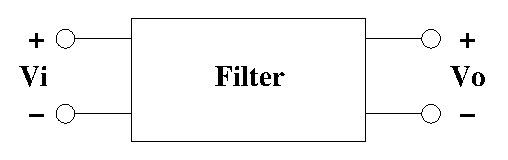
\includegraphics[width=0.4\linewidth]{hpf/hpf.eps}
\end{center}

You are designing a filter for a signal coming out of an ultrasound scanner.
The desired signal content ranges in frequency from 1-10 MHz, but there is
significant noise $\leq$ 100 Hz.  You must design a \underline{first-order}
filter that:

\begin{itemize}
\item Attenuates noise $\leq$ 100 Hz at least 40 dB below the desired
signal content (1-10 MHz), 
\item Does not distort the phase of the desired signal content (1-10 MHz) more than 15$^\circ$.
\end{itemize}

\begin{enumerate}
\item What type of filter do you need?  Why?
\vspace*{1.0in}
\item What is/are the cutoff frequency/frequencies of your filter?

\newpage
%{\bf BME154L - Spring 2012 - Exam \#2 Solutions}\hfill Name (Net ID):\underline{\hspace*{3.0in}}


\item Using 1 k$\Omega$ resistors and any value capacitors and/or inductors,
draw a circuit diagram, including component values, for your filter that
achieves the objectives described above.
\vspace*{3.0in}
\item Derive (don't just state) the transfer function ($H(j\omega)$) for your
filter.
\vspace*{2.5in}
\item Draw the Bode plot for your filter, including both magnitude and phase, labeling all important features and axes.

\newpage
%{\bf BME154L - Spring 2012 - Exam \#2 Solutions}\hfill Name (Net ID):\underline{\hspace*{3.0in}}


\vspace*{0.5in}
\centerline{\bf \Large Time-saver: Use your Bode plots from part (e)!!}

\item If your input signal is $V_i(t) = 100 \cos(2e6\pi t)$ V, then what is the
filter's output ($V_o(t)$)?  In addition to writing the expression for
$V_o(t)$, plot $V_o(t)$ below the plot of $V_i(t)$.  Remember to label the
voltage axis.  (Check yourself - this input signal should be in the passband of
your filter - remember the stated filter objectives.)

\hspace*{0.4\linewidth}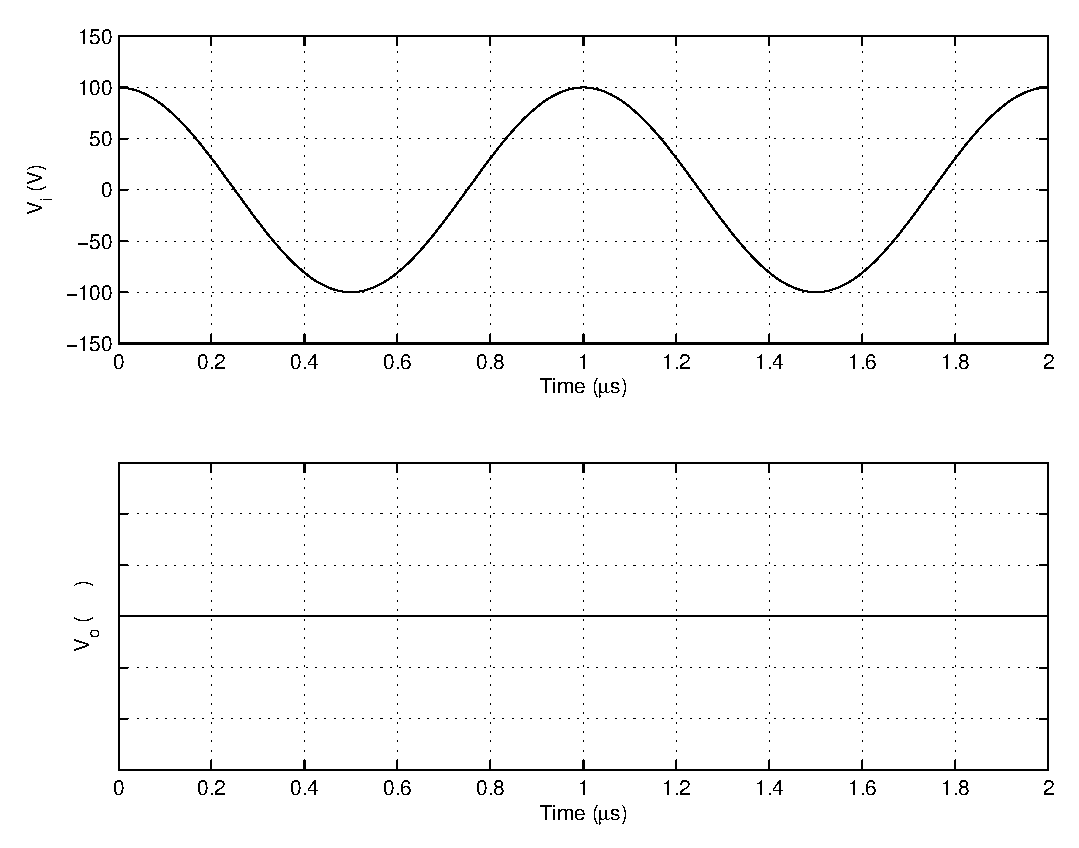
\includegraphics[width=0.6\linewidth]{hpf/plot_f.eps}

\vspace*{0.5in}

\item Repeat (f) for $V_i(t) = 100 \cos(200\pi t)$ V. (Check yourself - this
input signal should be in the noise band - remember the stated filter
objectives.)

\hspace*{0.4\linewidth}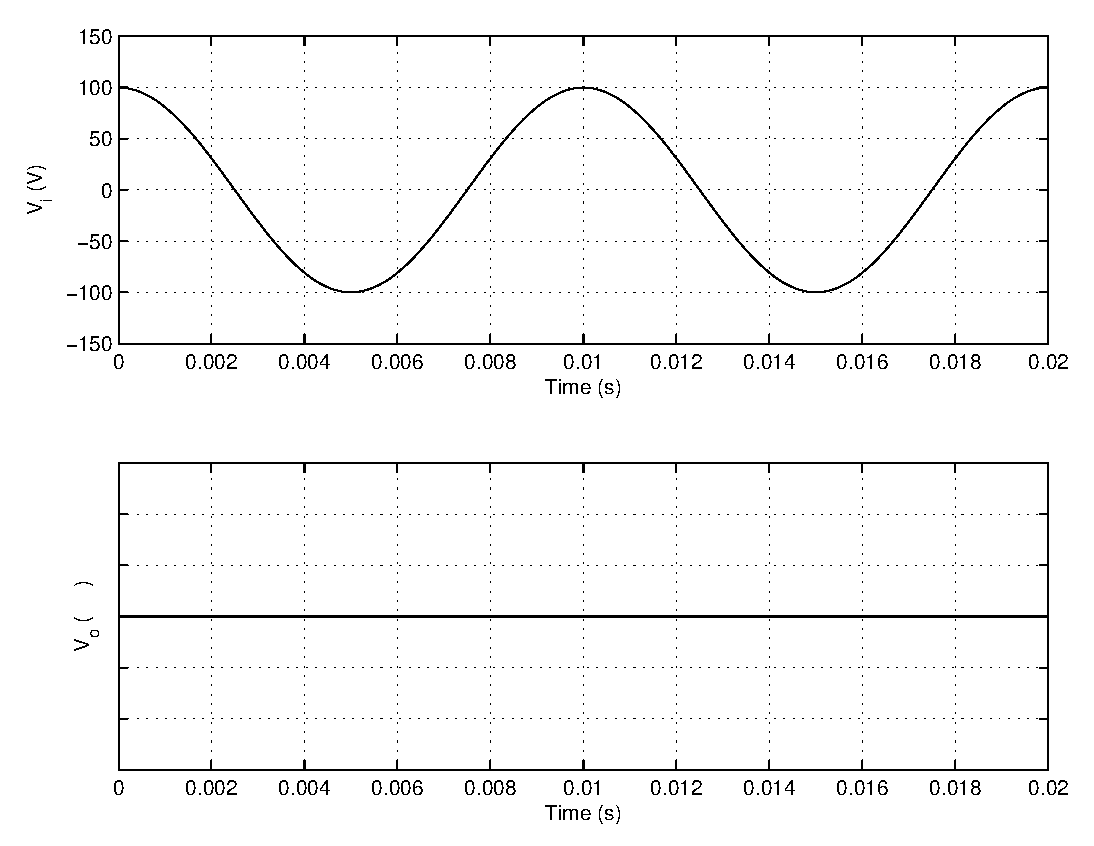
\includegraphics[width=0.6\linewidth]{hpf/plot_g.eps}
\end{enumerate}

\newpage
